    \chapter{Szczegółowy opis sterownika}
        Urządzenie wykonawcze jest głównym elementem całego systemu. Jest ono także najbardziej skomplikowanym fragmentem, a wynika to z wielu części składowych niezbędnych do przygotowania kompleksowego produktu. Składa się na niego między innymi projekt płytki drukowanej oraz projekt oprogramowania. Warto zaznaczyć że do skonstruowania w pełni autorskiego rozwiązania niezbędna jest szczegółowa wiedza z wielu dziedzin. Poczynając od elektroniki na programowaniu systemów wbudowanych kończąc.
    
    
        \section{Mikrokontroler}
            Jednostka obliczeniowa wybrana do przeprowadzania obliczeń mieści się w popularnym SoC (z angielskiego System on a chip) o oznaczeniu ESP32-WROOM-32UE \cite{esp_module}. SoC oznacza że na jednej małej płytce drukowanej znajduje się kilka sprzężonych ze sobą modułów. Takie rozwiązanie znacząco upraszcza konstrukcję nowych urządzeń ponieważ wszystkie krytyczne elementy są już rozmieszczone przez producenta SoC, który gwarantuje ich poprawne działanie.
            
            ESP32 jest to układ chińskiej firmy Espressif Systems \cite{espressif}. Został on wybrany ze względu na zintegrowany moduł WiFi oraz bardzo niską cenę wynoszącą poniżej 2\$ za sztukę, co perfekcyjnie wpisuje się w założenia projektu. Ponadto znajduje się w nim wiele ciekawych komponentów takich jak:
    
            \begin{itemize}
              \item dwurdzeniowy procesor o taktowaniu do 240MHz,
              \item 520 KiB RAM, 448 KiB ROM, 4 MB FLASH
              \item Bluetooth w standardzie 4.2 oraz BLE,
              \item 34 wyprowadzenia GPIO.
            \end{itemize}
            
            Użycie gotowego SoC znacznie upraszcza konstrukcję i gwarantuje poprawną współpracę zawartych w nim układów. Zainstalowany w nim mikrokontroler to ESP32-D0WD-V3. 
    
    
            \begin{figure}[ht]
              \centering
              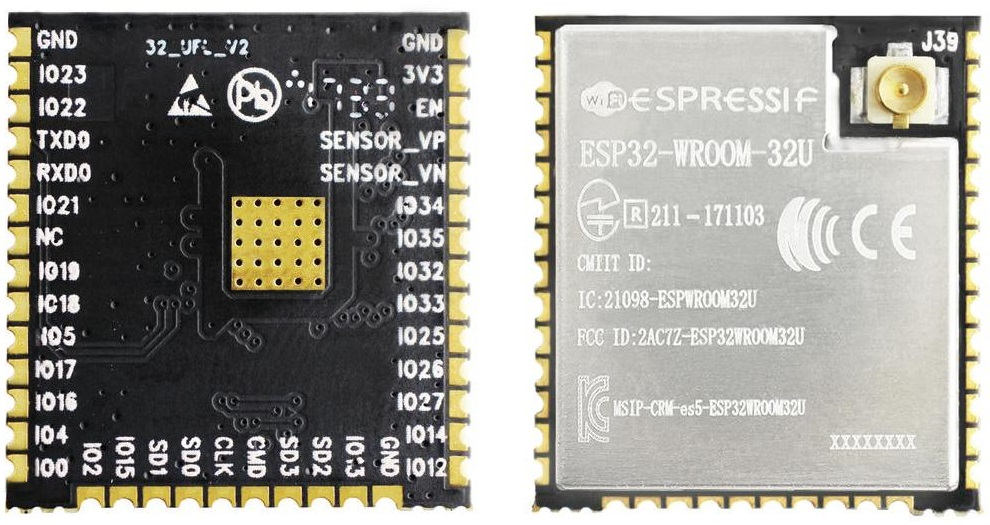
\includegraphics[width=0.4\textwidth]{img/esp32.jpg}
              \caption{Wykorzystana jednostka centralna \cite{esp_fig}}
              \label{esp}
            \end{figure}
    
    
        \section{System operacyjny}
            Jednym z wielu wyzwań stawianych przed programistą systemów wbudowanych jest stworzenie rozbudowanego programu wykonującego wiele zadań na pojedynczej jednostce obliczeniowej. Powoduje to konieczność wykorzystywania rozbudowanych maszyn stanów i bardzo skomplikowanej logiki. Z pomocą przychodzą systemy operacyjne, które umożliwiają tworzenie programów wielowątkowych i uprzyjemniają korzystanie z procesorów wielordzeniowych. Ze względu na to że użyty w projekcie procesor ma dwa rdzenie logiczne oraz że program ten powinien wykonywać wiele czynności jednocześnie, zdecydowano się skorzystać z funkcjonalności oferowanej przez systemy operacyjne. 
            
            Program wykonuje się więc pod kontrolą otwarto źródłowego systemu czasu rzeczywistego FreeRTOS \cite{freertos}. Jest on znany z dużej szybkości działania. Implementuje on wszystkie elementy niezbędne do pracy z wieloma procesami takie jak muteksy, semafory czy kolejki priorytetowe. Bez niego obsługa WiFi czy protokołu MQTT byłaby zdecydowanie bardziej skomplikowana i czasochłonna. 
            
            \vspace{1em}
            
            \begin{figure}[ht]
              \centering
              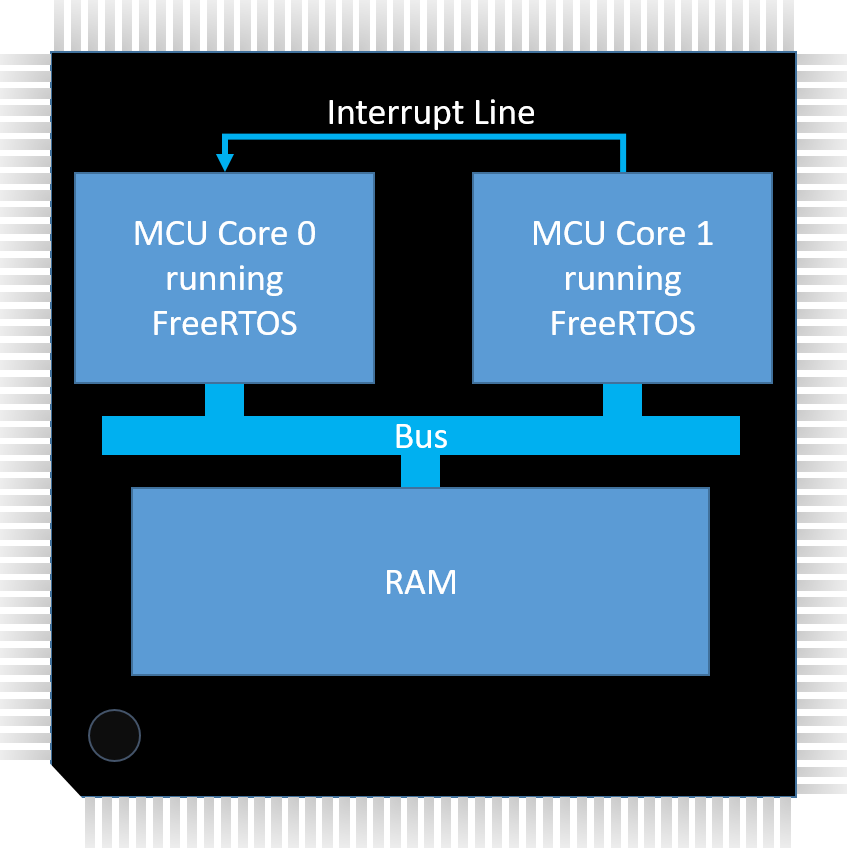
\includegraphics[width=0.5\textwidth]{img/multicore_amp_hardware_configuration.png}
              \caption{Topologia procesora z użyciem FreeRTOS \cite{freertos_fig}}
              \label{freertos}
            \end{figure}
            
            \vspace{1em}
            
            Mówiąc o zaletach systemów operacyjnych warto też wspomnieć o ich wadach. Najważniejszą z nich jest narzut obliczeniowy wynikający między innymi z pracy planisty oraz przełączania kontekstów. Z tego powodu część czasu procesora poświęcana jest na pracę samego systemu i nie bierze udziału w wykonywaniu obliczeń na rzecz programu. Należy zaznaczy że nie są to duże wartości i są one zależne od indywidualnej konfiguracji systemu operacyjnego. W przytoczonym przez dokumentację FreeRTOS przykładzie \cite{context} przełączenie kontekstu zajmuje 84 cykle procesora, co jest bardzo małą wartością biorąc pod uwagę taktowanie na poziomie 240MHz. Z tego powodu systemy operacyjne znajdują szerokie zastosowanie nie tylko w zastosowaniach profesjonalnych, bo dzięki prostocie FreeRTOS, jest on coraz to częściej wykorzystywanych przez amatorów i hobbistów.
            
        \subsection{Szeregowanie zadań}
            Ważnych aspektem funkcjonowania systemu operacyjnego jest współbieżność procesów. Każdy z nich posiada swój priorytet oraz aktualny stan. Możliwe stany w systemie FreeRTOS zostały przedstawione na rysunku \ref{fig:freertos_tasks_state}.
      
            \begin{figure}[ht]
              \centering
              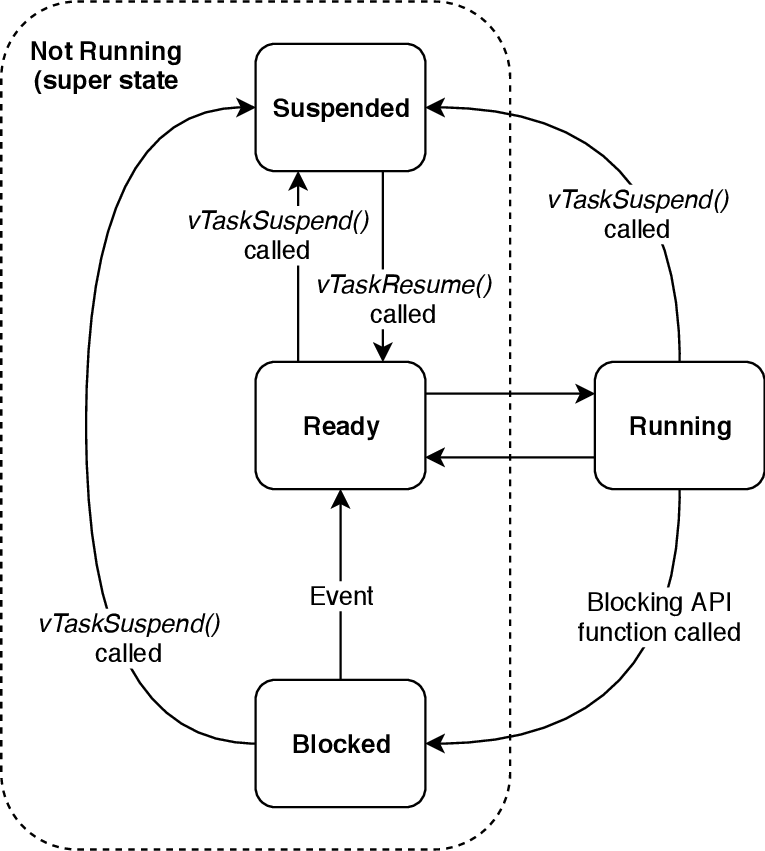
\includegraphics[width=0.6\textwidth]{img/FreeRTOS-tasks-state.png}
              \caption{Możliwe stany procesów w FreeRTOS \cite{freertos_task_fig}}
              \label{fig:freertos_tasks_state}
            \end{figure}
            
            Zadania w stanie gotowości szeregowane są względem ustawionego priorytetu. W przypadku znalezienia się kilku zadań o identycznym priorytecie, są one szeregowane według algorytmu karuzelowego (z ang. Round Robin \cite{round_robin}).
            
        \section{Framework}
            Przy opracowywaniu kodu źródłowego sterownika został użyty framework ESP-IDF \cite{esp-idf} przygotowany przez producenta procesora. Na stronie dostawcy tego rozwiązania można znaleźć także obszerną dokumentację tłumaczącą wykorzystanie frameworka w praktyce wraz z wieloma przykładami użycia. Zastosowanie gotowej abstrakcji zdejmuje z dewelopera obowiązek implementacji wielu skomplikowanych aspektów programu. W tym projekcie szczególnie przydatna jest implementacja stosu TCP/IP i protokołu MQTT.
    
    
        \section{Kolejki i wątki}
            \subsection{Opis}
            Największą zaletą posiadania systemu operacyjnego jest możliwość tworzenia osobnego procesu dla każdego zadania. To znowu pozwala dokładnie kontrolować czasy wywołań i częstotliwości odpowiednich wydarzeń. Główne zadania stawiane temu sterownikowi to:
            
            \begin{itemize}
                \item obsługa silnika wraz z liczeniem PID,
                \item pomiary napięcia zasilania,
                \item wysyłanie danych przez MQTT,
                \item obsługa WiFi, odbieranie danych z MQTT, planista i obsługa przerwań
            \end{itemize}
            
            W ten sposób kształtują się cztery główne procesy, które biorą udział w pracy systemu:
            
            \begin{description}
                \item [Główny] Jest głównym procesem w systemie. Odpowiada on za początkową konfigurację peryferiów przy starcie systemu. Z niego powstaje także reszta procesów. Po poprawnym starcie zajmuje się on obsługą połączenia z siecią, klientem MQTT, przerwaniami oraz planistą systemu. 
                
                \item [PID] Proces PID wykonuje się dokładnie co 10ms. Każde odchylenie w czasie tego procesu powodowałoby niedokładną pracę regulatora PID, co skutkowałoby niestabilnym zachowaniem się silnika. Z tego też powodu, ten proces został na stałe powiązany do drugiego rdzenia procesora oraz otrzymał bardzo wysoki priorytet. Jego schemat działania został zamieszczony na rys. \ref{fig:pid_plantuml} 
                
                \item [ADC] Proces ADC odpowiedzialny jest za pomiary zasilania. Wykonuje się co około 20ms, ale ze względu na ustawiony bardzo niski priorytet ustępuje każdemu innemu zadaniu. Wykonuje się więc tylko gdy procesor nic innego nie robi. Nie stanowi to żadnego problemu, ponieważ opóźnienia w wykonywaniu tego procesu nie wpływają z znacznym stopniu na prawidłową pracę systemu. Informacja przez niego generowana trafia wyłącznie na panel kontrolny użytkownika i jest wyświetlana w aplikacji dostępowej, gdzie aktualizowana jest z częstotliwością około 5Hz. Drobne odchyłki w czasie aktualizacji są więc niewykrywalne. Proces ten został przypięty do rdzenia pierwszego.
                
                \item [WiFi] Proces WiFi. Rola tego procesu jest bardzo skromna i ogranicza się jedynie do inicjalizacji połączenia z WiFi. Po wykonaniu tego zadania proces ten się kończy, a rolę obsługi połączenia bezprzewodowego przejmuje proces systemowy.
                
                \item [MQTT] Zadaniem procesu MQTT jest odbieranie danych z kolejek priorytetowych FIFO i wysyłanie ich do brokera. Otrzymał on średni priorytet. Wykonuje się w momencie gdy, w którejś z kolejek pojawiają się jakieś nowe dane. On również został przypisany do rdzenia pierwszego.
                
            \end{description}
            
            \begin{figure}[ht]
                \centering
                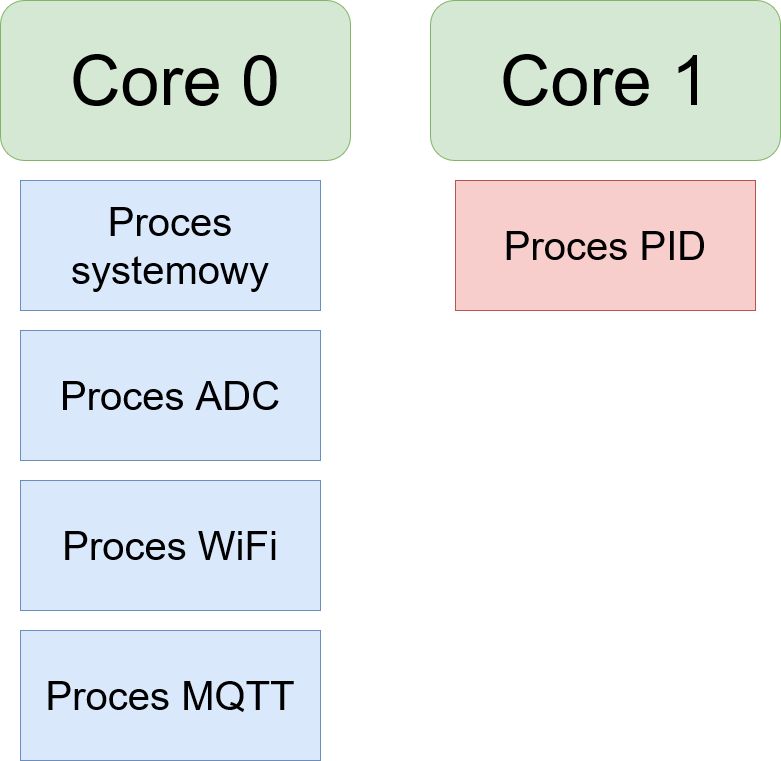
\includegraphics[width=0.8\textwidth]{img/task_diagram.png}
                \caption{Diagram wątków}
                \label{fig:task_diagram}
            \end{figure}
            
            \subsection{Implementacja menadżera wątków}
            Został stworzony specjalny moduł odpowiedzialny za zarządzanie wątkami. Pozwala to na łatwe dodawanie i usuwanie funkcjonalności z systemu. Dodanie nowego procesu ogranicza się do wypełnienia struktury przedstawionej na listingu \ref{code:task_struct}, a następnie dopisania kolejnej pozycji w liście z listingu \ref{code:task_list}.
            
            \begin{kod}
              \inputminted[firstline=12, lastline=22]{cpp}{esp/listings/task_mngm.hpp}
              \caption{Struktura konfiguracyjna wątku}
              \label{code:task_struct}
              \vspace{2em}
            \end{kod}
            
            \begin{kod}
              \inputminted[firstline=25, lastline=32]{cpp}{esp/listings/task_mngm.hpp}
              \caption{Lista wątków}
              \label{code:task_list}
              \vspace{2em}
            \end{kod}
            
            Implementacja wątków zawartych w systemie przedstawiona została na listingu \ref{code:task_config}. Jest to tablica wcześniej wspomnianych struktur. Pierwsze pole struktury jest uchwytem do wybranej funkcji. Następnie należy podać nazwę procesu. Jest to niezwykle przydatne przy szukaniu błędów, ponieważ nazwa ta jest używana podczas wypisywania informacji diagnostycznych. Kolejne pola to wielkość stosu, przekazywane parametry, priorytet wykonywania, uchwyt do procesu oraz numer rdzenia który ma zajmować się obsługą konfigurowanego zadania.
            
            \begin{kod}
              \inputminted[firstline=19, lastline=60]{cpp}{esp/listings/task_mngm.cpp}
              \caption{Konfiguracja wątków}
              \label{code:task_config}
              \vspace{2em}
            \end{kod}
            
            \subsection{Implementacja menadżera kolejek}
            Zastosowanie kolejek priorytetowych umożliwia komunikację między procesami. Można je deklarować i inicjalizować w modułach, które polegają na przesyłanych danych, ale sprowadza to znaczny bałagan w kodzie. Dużo lepszym rozwiązaniem jest umieszczenie ich w jednym module, który zadba o ich konfigurację i inicjalizację. Zostało to zaprojektowane w sposób bliźniaczy do menadżera wątków. Podstawą jest struktura pokazana w listingu \ref{code:queue_struct}.
 
            \begin{kod}
              \inputminted[firstline=40, lastline=47]{cpp}{esp/listings/task_mngm.hpp}
              \caption{Struktura konfiguracyjna kolejki}
              \label{code:queue_struct}
              \vspace{2em}
            \end{kod}
            
            Struktura ta zawiera uchwyt do kolejki, wielkość transportowanego elementu, dopuszczalną ilość elementów w kolejce oraz nazwę. Przykład wykorzystania został przedstawiony w listingu \ref{code:queue_config}. 
            
            \begin{kod}
              \inputminted[firstline=63, lastline=99]{cpp}{esp/listings/task_mngm.cpp}
              \caption{Konfiguracja kolejek FIFO}
              \label{code:queue_config}
              \vspace{1em}
            \end{kod}
            
            Uchwyty do kolejek są przypisywane podczas inicjalizacji kolejek. Kod dotyczący inicjalizacji umieszczony jest pod listingiem \ref{code:queue_init}.
            
             \begin{kod}
              \inputminted[firstline=235, lastline=242]{cpp}{esp/listings/task_mngm.cpp}
              \caption{Inicjalizacja kolejek FIFO}
              \label{code:queue_init}
              \vspace{1em}
            \end{kod}          
            
            Wykorzystanie kolejek poza modułem byłoby mocno utrudnione bez zdefiniowania odpowiednich makr, które odnoszą się do przypisanych uchwytów. Kod znajduje się w listingu \ref{code:queue_define}.
            
             \begin{kod}
              \inputminted[firstline=63, lastline=71]{cpp}{esp/listings/task_mngm.hpp}
              \caption{Makra do uchwytów kolejek FIFO}
              \label{code:queue_define}
              \vspace{2em}
            \end{kod} 
            
            
        \section{Mostek H}
            Głównym zadaniem mikrokontrolerów jest zbieranie danych z czujników, wykonywanie obliczeń i podejmowanie decyzji. Nie zostały jednak stworzone do sterowania elementami o wyższym napięciu czy dużych prądach, ponieważ takie wymagania znacznie utrudniają miniaturyzację. Z tego powodu wyjścia mikrokontrolerów potrafią dostarczyć zazwyczaj około kilkudziesięciu miliamperów prądu. W przypadku mikrokontrolera użytego w projekcie dokumentacja \cite{esp32} informuje o bardzo wysokim prądzie wyjściowym dochodzącym nawet do 40mA w sprzyjających warunkach. Jest to wystarczające natężenie prądu do zasilenia diody LED (ok. 20mA) czy sterowania tranzystorem. Z drugiej strony jest to wielokrotnie za mało, aby uruchomić silnik prądu stałego. Takie silniki zazwyczaj nie dość że działają na znaczenie wyższych napięciach niż 3.3V to często potrafią także zużyć ponad 2A prądu podczas obciążenia. Jednym ze sposobów kontrolowania prędkości obrotowej takiego jest zastosowanie wcześniej wspomnianego tranzystora lub przekaźnika, ale minusem takiego rozwiązania jest brak możliwości zmiany kierunku obrotów. Z tego powodu najczęściej stosowanym rozwiązaniem, które pozwoli na sterowanie silnikiem w obu kierunkach jest użycie mostka H. Jego schemat przedstawiono na rys. \ref{fig:h_bridge_schematic}.
            
            \begin{figure}[ht]
                \centering
                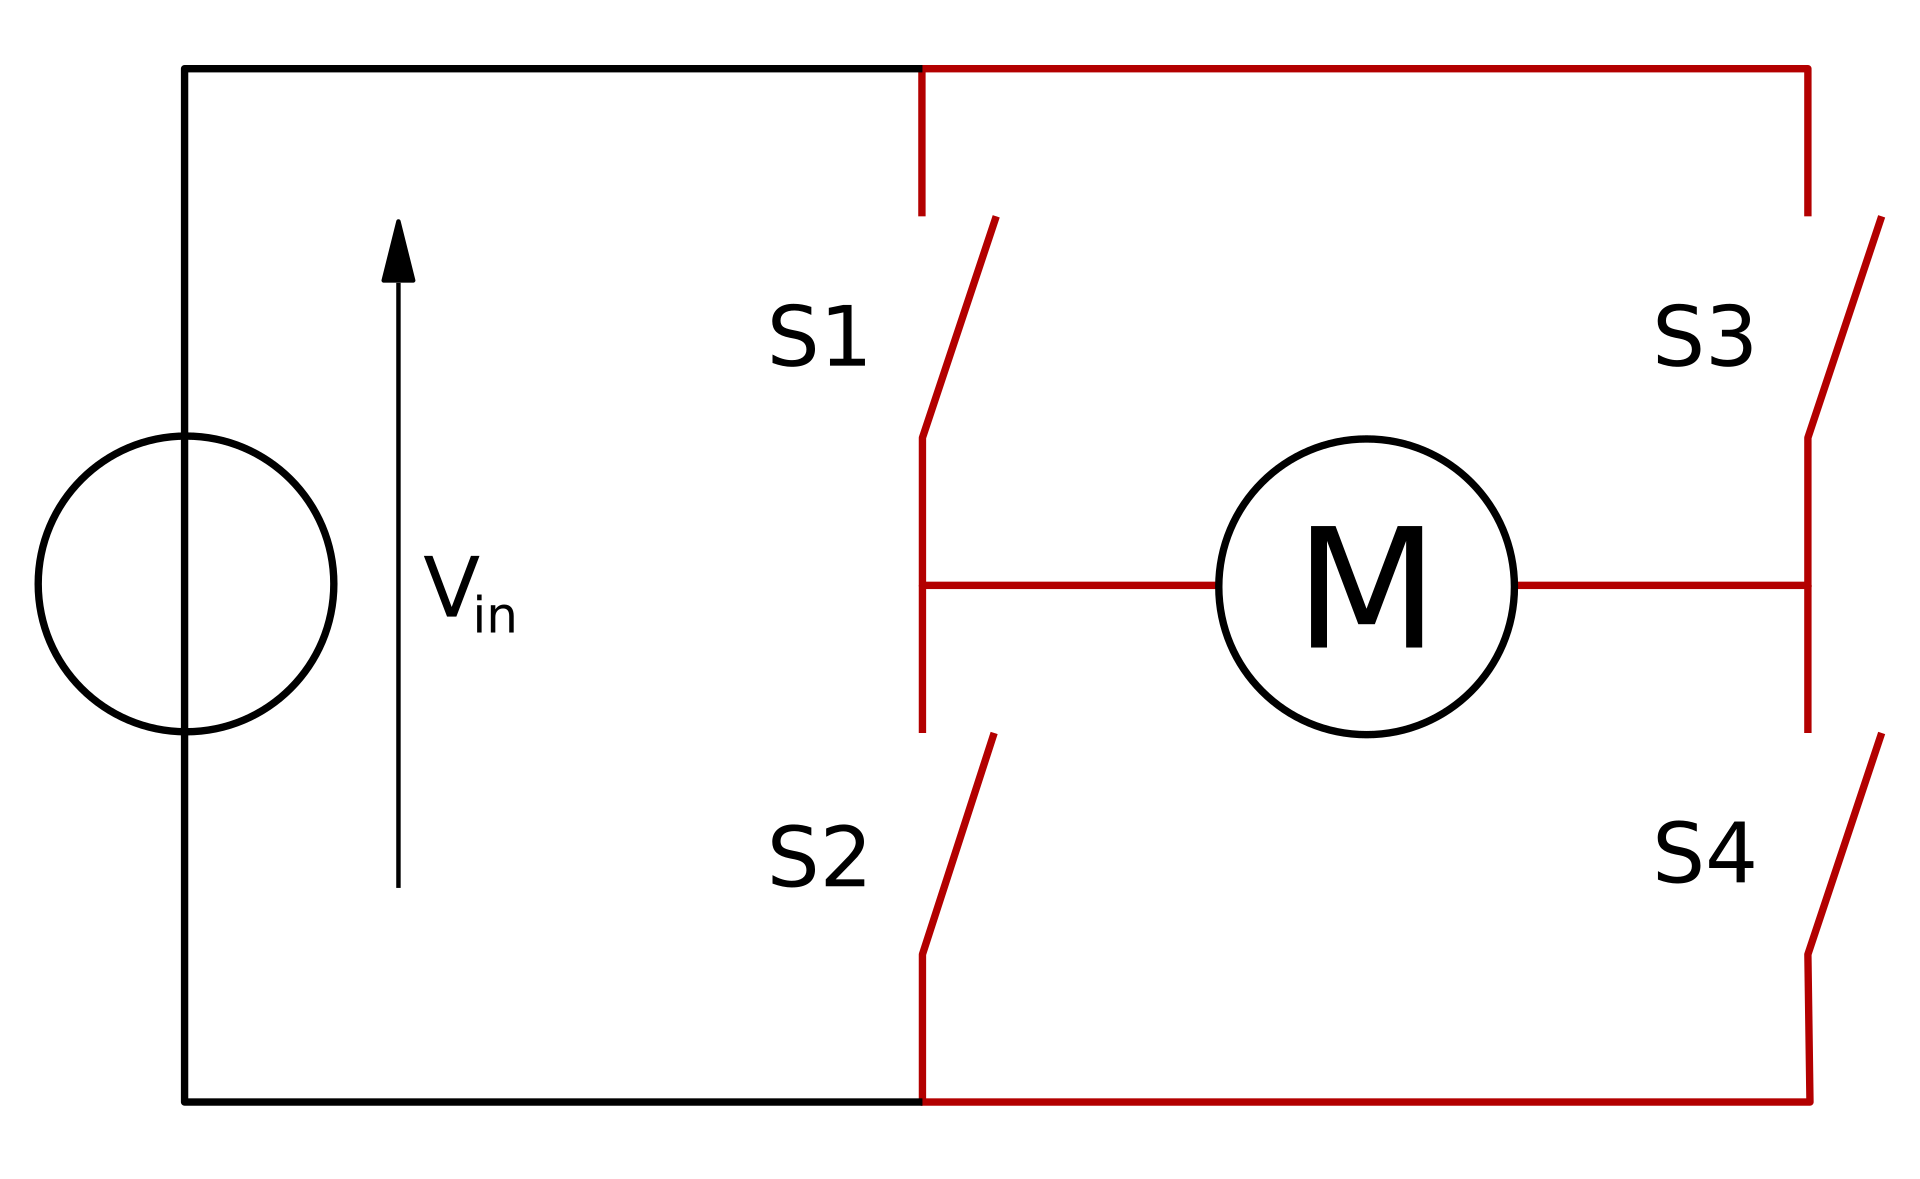
\includegraphics[width=0.7\textwidth]{img/h_bridge_schametic.png}
                \caption{Ogólny schemat mostka H \cite{h_bridge_conn_fig}}
                \label{fig:h_bridge_schematic}
            \end{figure}
            
            W roli mostka H został wyselekcjonowany bardzo popularny układ scalony L298N w obudowie Multiwatt15. Nie jest to nowy układ scalony, ale jest on przetestowany i zdecydowanie wystarczający dla tego zastosowania. Może się on poszczycić napięciem zasilania silników do 46V i prądem szczytowym na poziomie 2A. W rzeczywistości posiada on dwa osobne kanały, co sprawia że z jego pomocą możliwe jest jednoczesne sterowanie dwoma silnikami. Jednakże projekt ten zakłada wykorzystanie tylko jednego silnika, więc drugi kanał pozostanie nieaktywny. Może to spowodować pozytywny wpływ na wolniejsze nagrzewanie się układu, co z pewnością przełoży się na jego stabilniejszą pracę. 
            
            Układ scalony zastosowany w projekcie został przedstawiony na rys. \ref{fig:h_bridge}. Redukuje on znacząco poziom skomplikowania urządzenia ponieważ w celu uruchomienia go wystarczą cztery diody redukujące prądy indukowane na cewkach silników podczas ich pracy oraz kondensator filtrujący zasilanie \cite{mostek}. Przykładowe podłączenie jest zaprezentowane na rys. \ref{fig:h_bridge_connection}.
            
            \begin{figure}[ht]
                \centering
                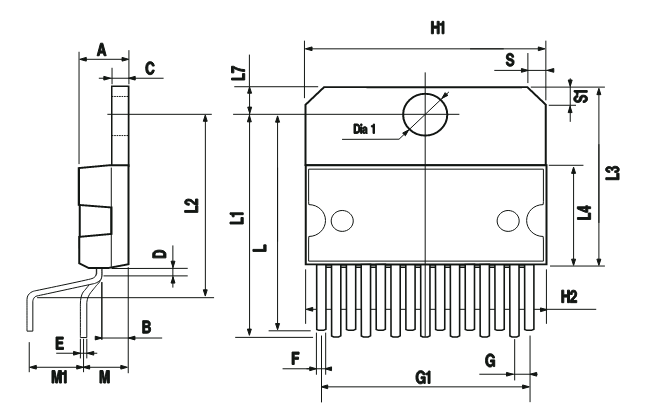
\includegraphics[width=0.7\textwidth]{img/h_bridge.png}
                \caption{Schemat wykorzystanego mostka H \cite{h_bridge_fig}}
                \label{fig:h_bridge}
            \end{figure}
            
            \begin{figure}[ht]
                \centering
                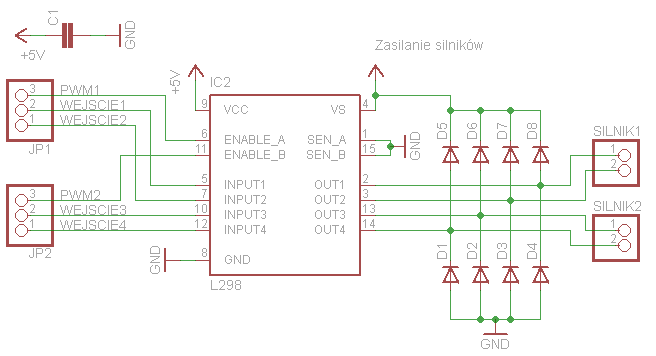
\includegraphics[width=0.7\textwidth]{img/h_bridge_connection.png}
                \caption{Schemat podłączenia mostka H \cite{h_bridge_conn_fig}}
                \label{fig:h_bridge_connection}
            \end{figure}
            
        \section{Silnik}
            Silnik jest to bardzo konkurencyjnie wyceniany produkt firmy DFROBOT. Został on wybrany w głównej mierze ze względu na swoją niską cenę i parametry, które w zupełności wystarczą do zrealizowania tego projektu. Jest on wyposażony w metalową przekładnię zapewniającą przełożenie napędu w proporcji 20:1. Ponadto, na końcu silnika znajduje się fabrycznie zamontowany enkoder kwadraturowy, który produkuje 11 impulsów na każdy obrót wałka głównego. Schemat silnika wraz z enkoderem umieszczony został na rys. \ref{fig:engine}
            
            \begin{figure}[ht]
                \centering
                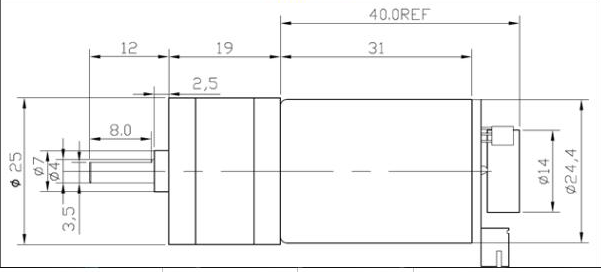
\includegraphics[width=0.9\textwidth]{img/silnik.png}
                \caption{Schemat wykorzystanego silnika \cite{engine_fig}}
                \label{fig:engine}
            \end{figure}


        \section{Płytka PCB}
            \subsection{Opis}
                Urządzenie wykonawcze zawiera mikrokontroler, mostek H oraz element wykonawczy w postaci silnika prądu stałego wyposażonego w enkoder kwadraturowy. Poza możliwością zadawania napięcia na silnik, urządzenie dysponuje funkcją pomiaru napięcia zasilania. Poza wymienionymi jednostkami na płytce drukowanej znajdują się także wszystkie elementy niezbędne do prawidłowej pracy procesora takie jak kondensatory i rezystory.
          
            \subsection{Wygląd}
                Przygotowany wzór płytki drukowanej z rozlokowanymi elementami i poprowadzonymi ścieżkami został złączony do tego dokumentu. Obie strony płytki zarówno górna jak i dolna dostępne są jako rysunek \ref{fig:pcb}.
                
                \begin{figure}[ht]
                    \centering
                    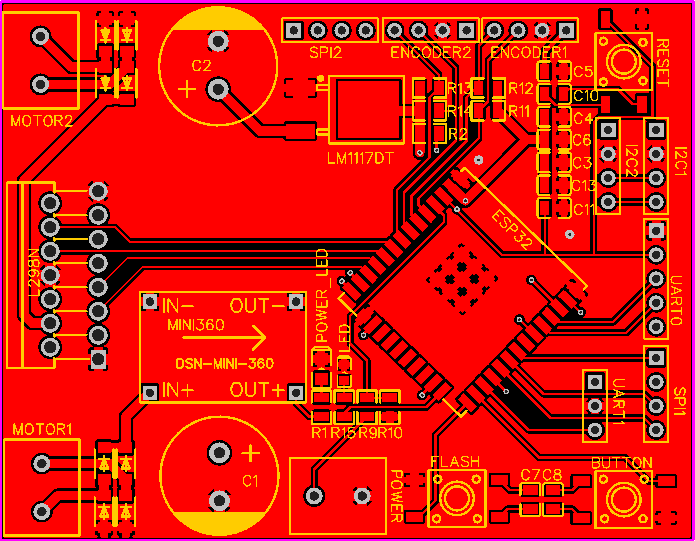
\includegraphics[width=0.8\textwidth]{img/pcb_front.png}
                    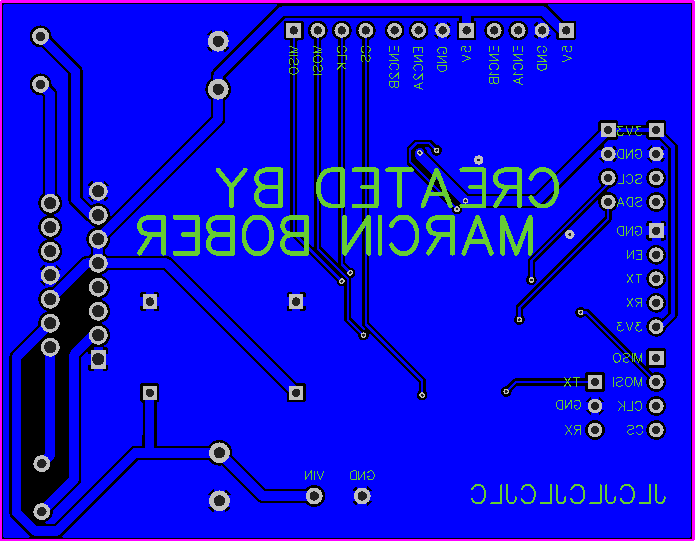
\includegraphics[width=0.8\textwidth]{img/pcb_back.png}
                    \caption{Wygląd PCB}
                    \label{fig:pcb}
                \end{figure}
    
            \subsection{Schemat}
                Schemat składa się z trzech stron. Pierwsza strona (rys. \ref{fig:pcb_schematic_1}) dotyczy sekcji zasilania oraz połączeń z SoC wraz z elementami niezbędnymi do jego prawidłowej pracy. Druga strona (rys. \ref{fig:pcb_schematic_2}) opisuje połączenia enkoderów oraz mostka H. Trzecia strona (rys. \ref{fig:pcb_schematic_3}) są to jednie wyprowadzenia interfejsów.
                  
                \begin{landscape}
                    \begin{figure}
                      \centering
                      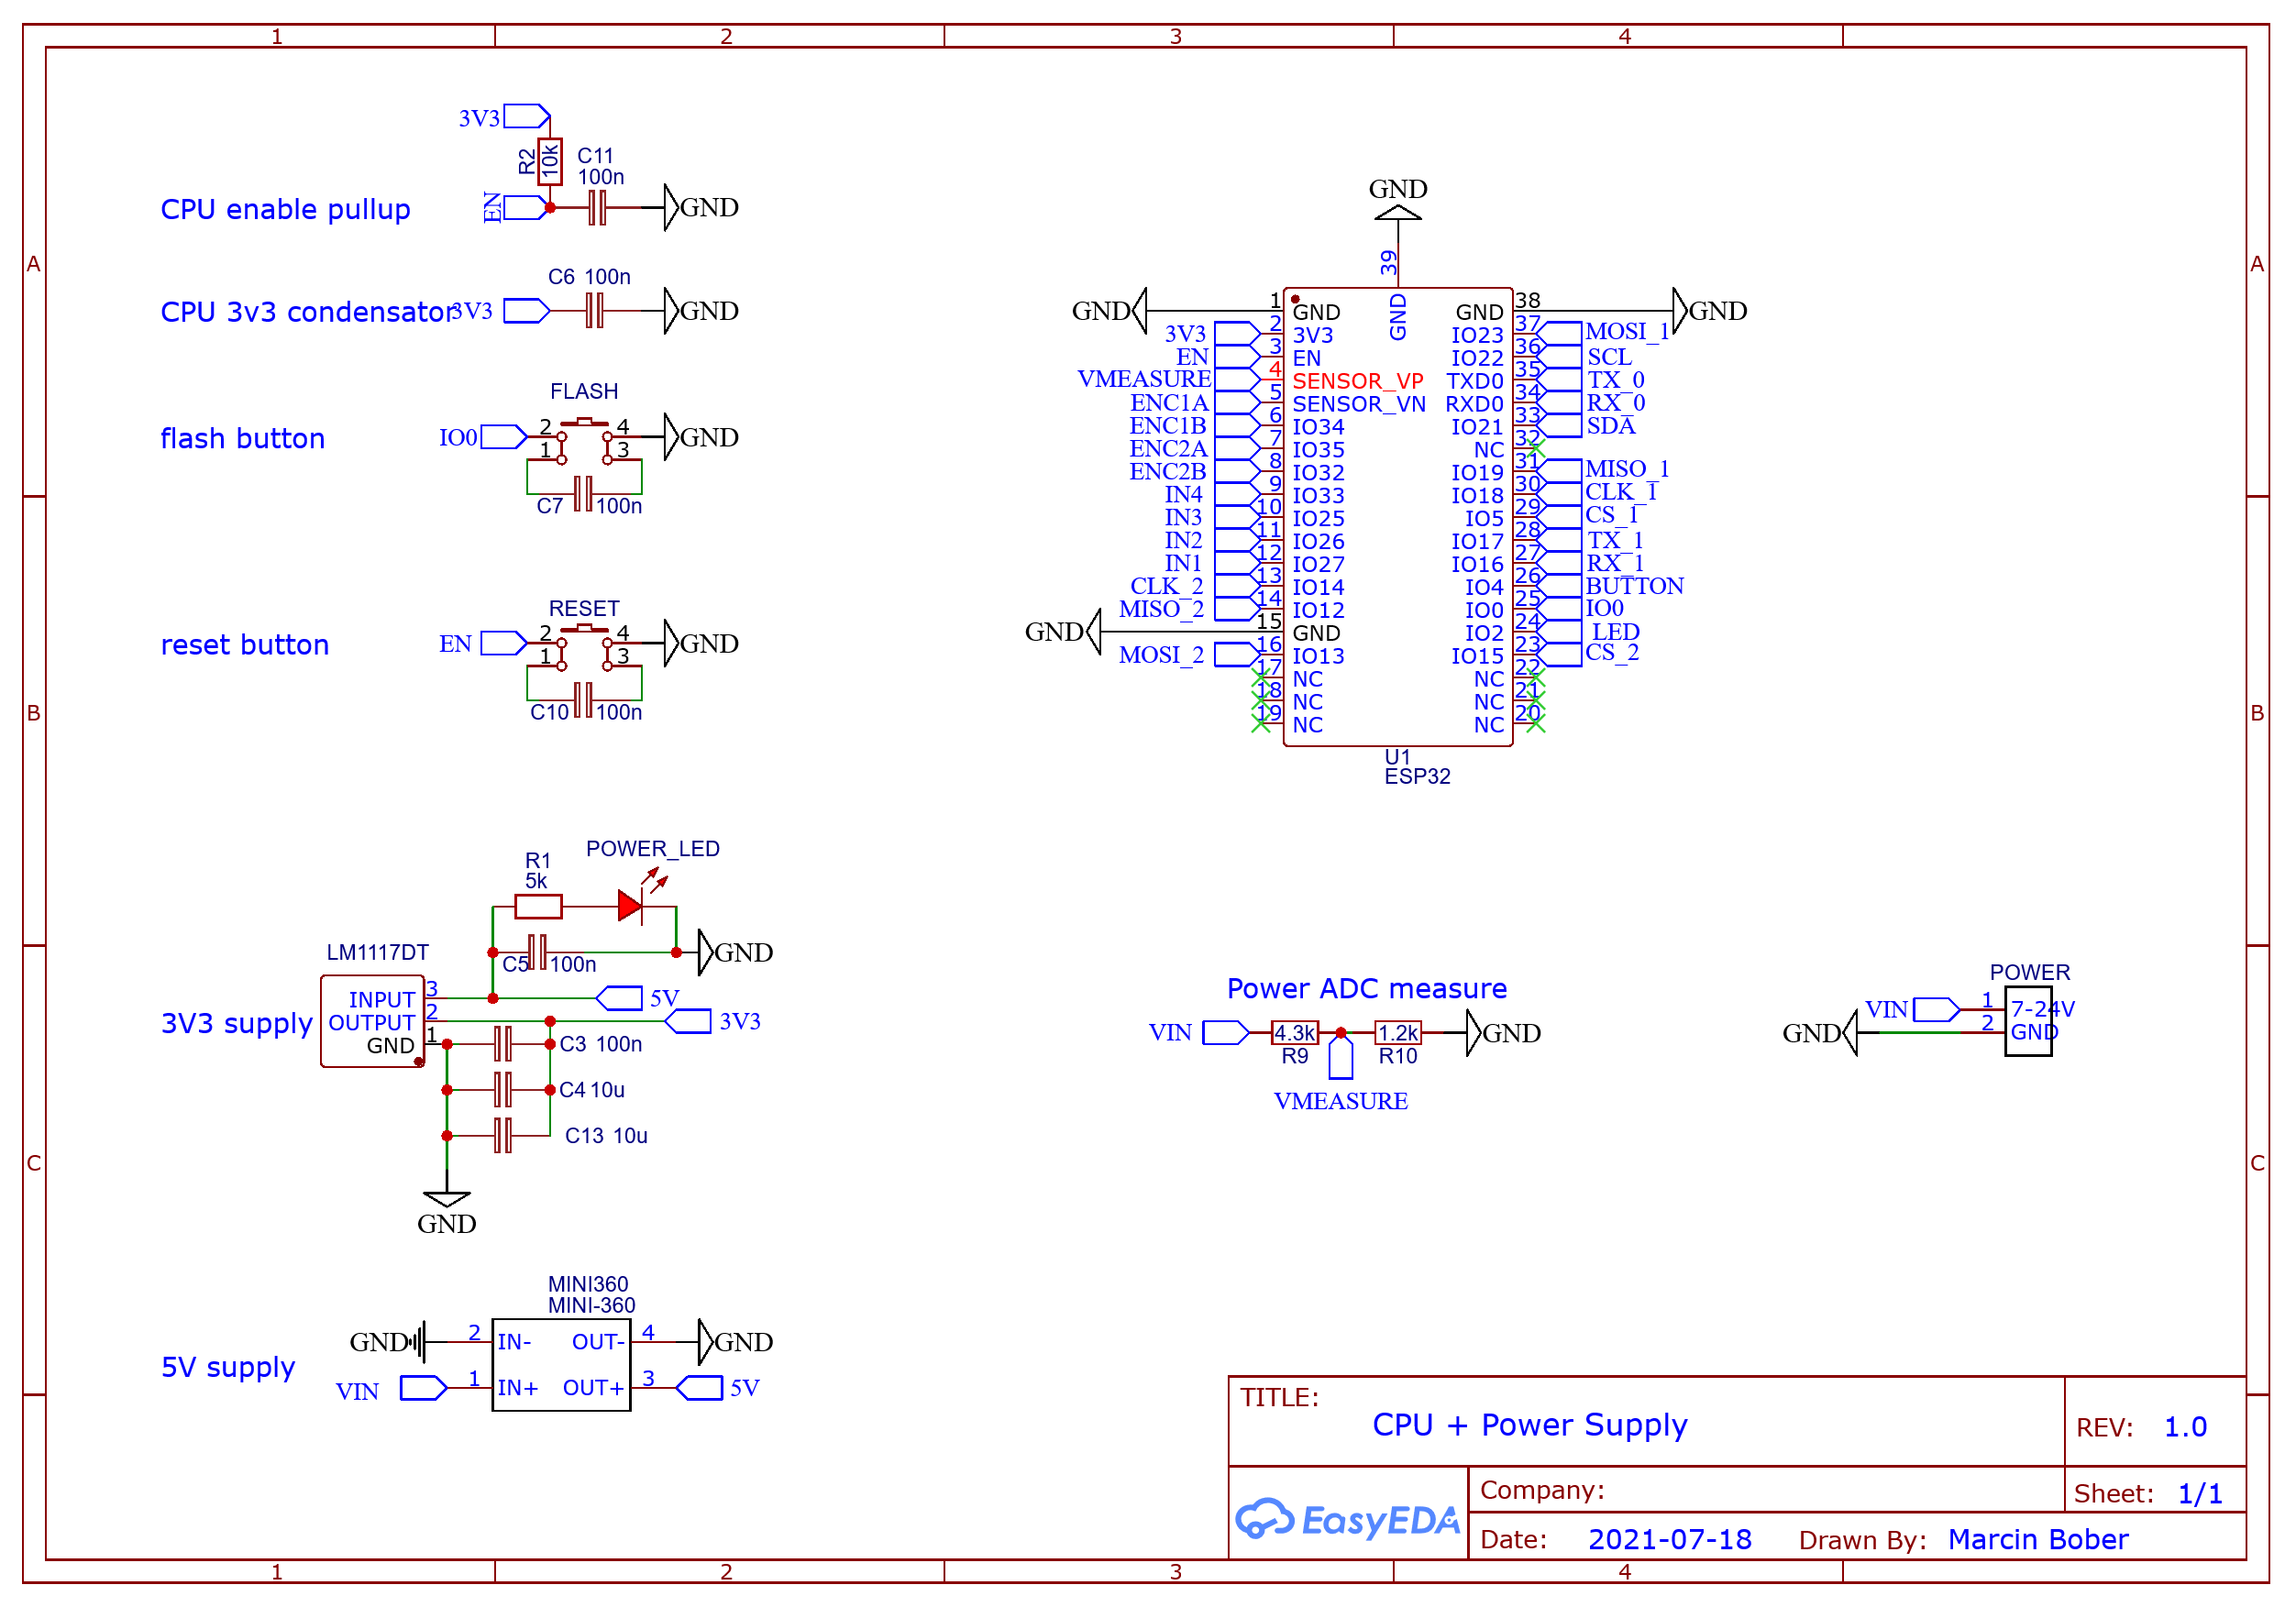
\includegraphics[width=0.85\textwidth]{img/pcb1.png}
                      \caption{Schemat płytki PCB (CPU+PSU)}
                      \label{fig:pcb_schematic_1}
                    \end{figure}
                \end{landscape}
                
                \begin{landscape}
                    \begin{figure}
                      \centering
                      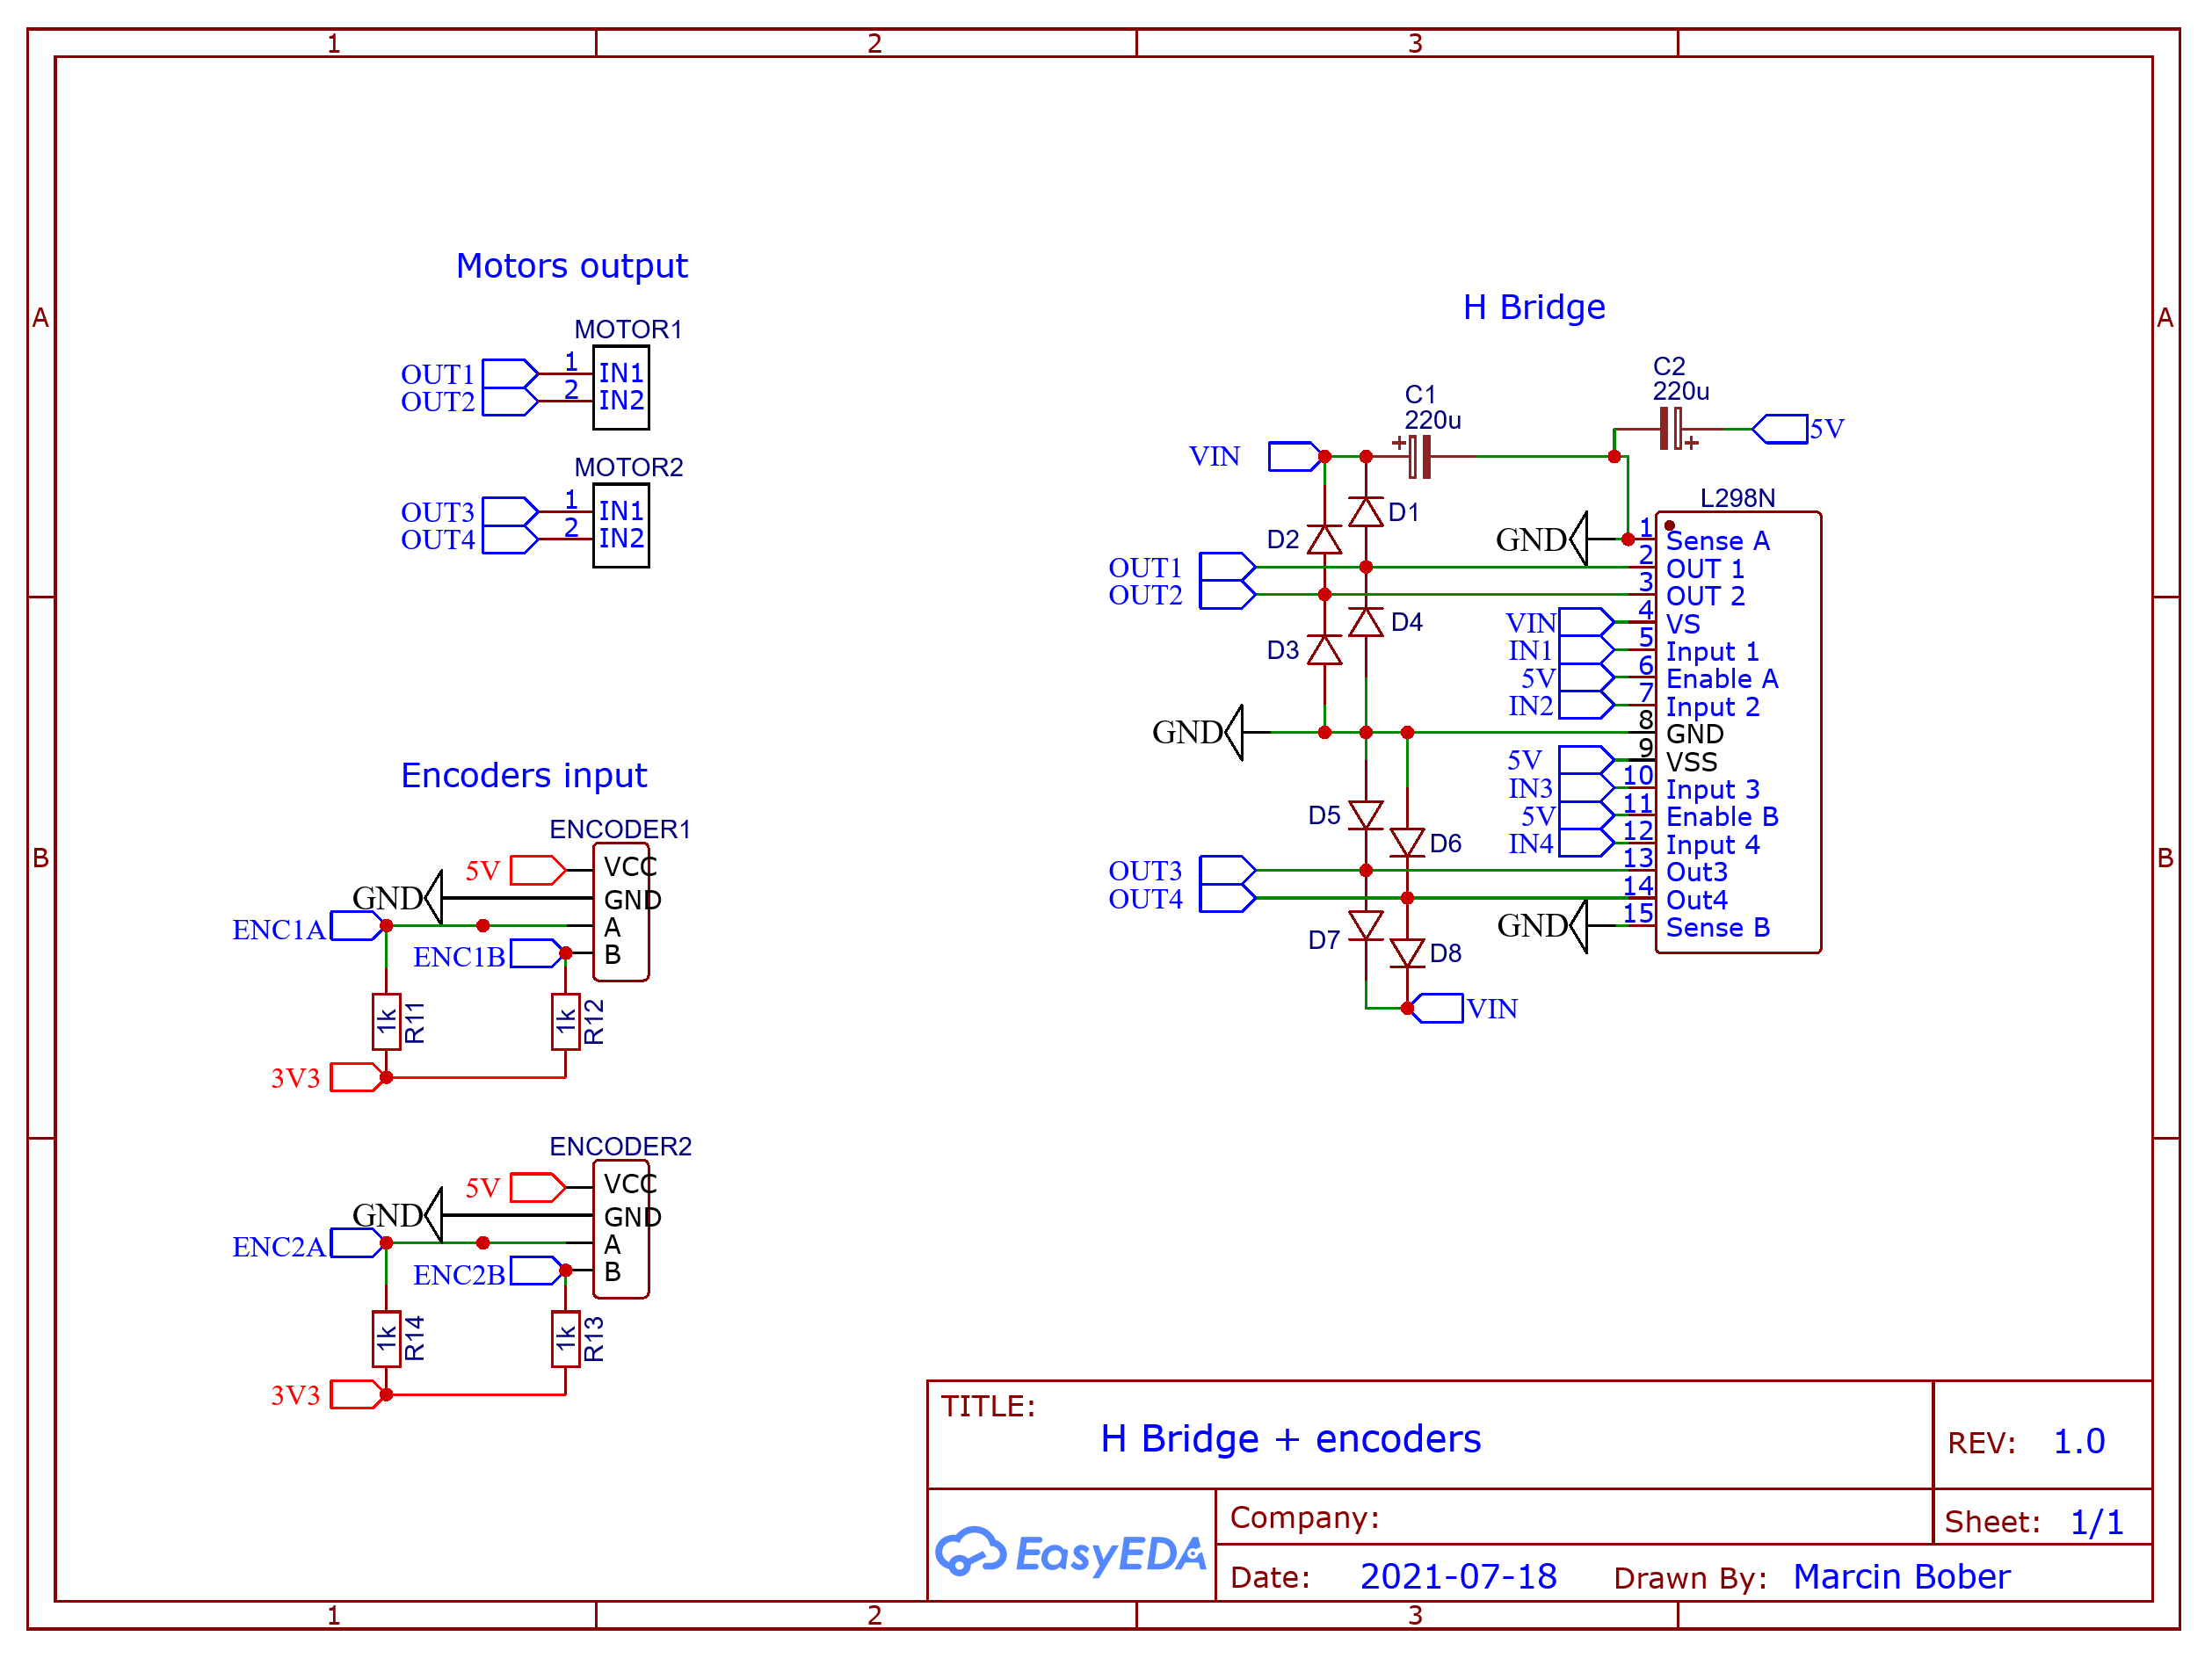
\includegraphics[width=0.80\textwidth]{img/pcb2.png}
                      \caption{Schemat płytki PCB (mostek + enkodery)}
                      \label{fig:pcb_schematic_2}
                    \end{figure}
                \end{landscape}
        
                \begin{landscape}
                    \begin{figure}
                      \centering
                      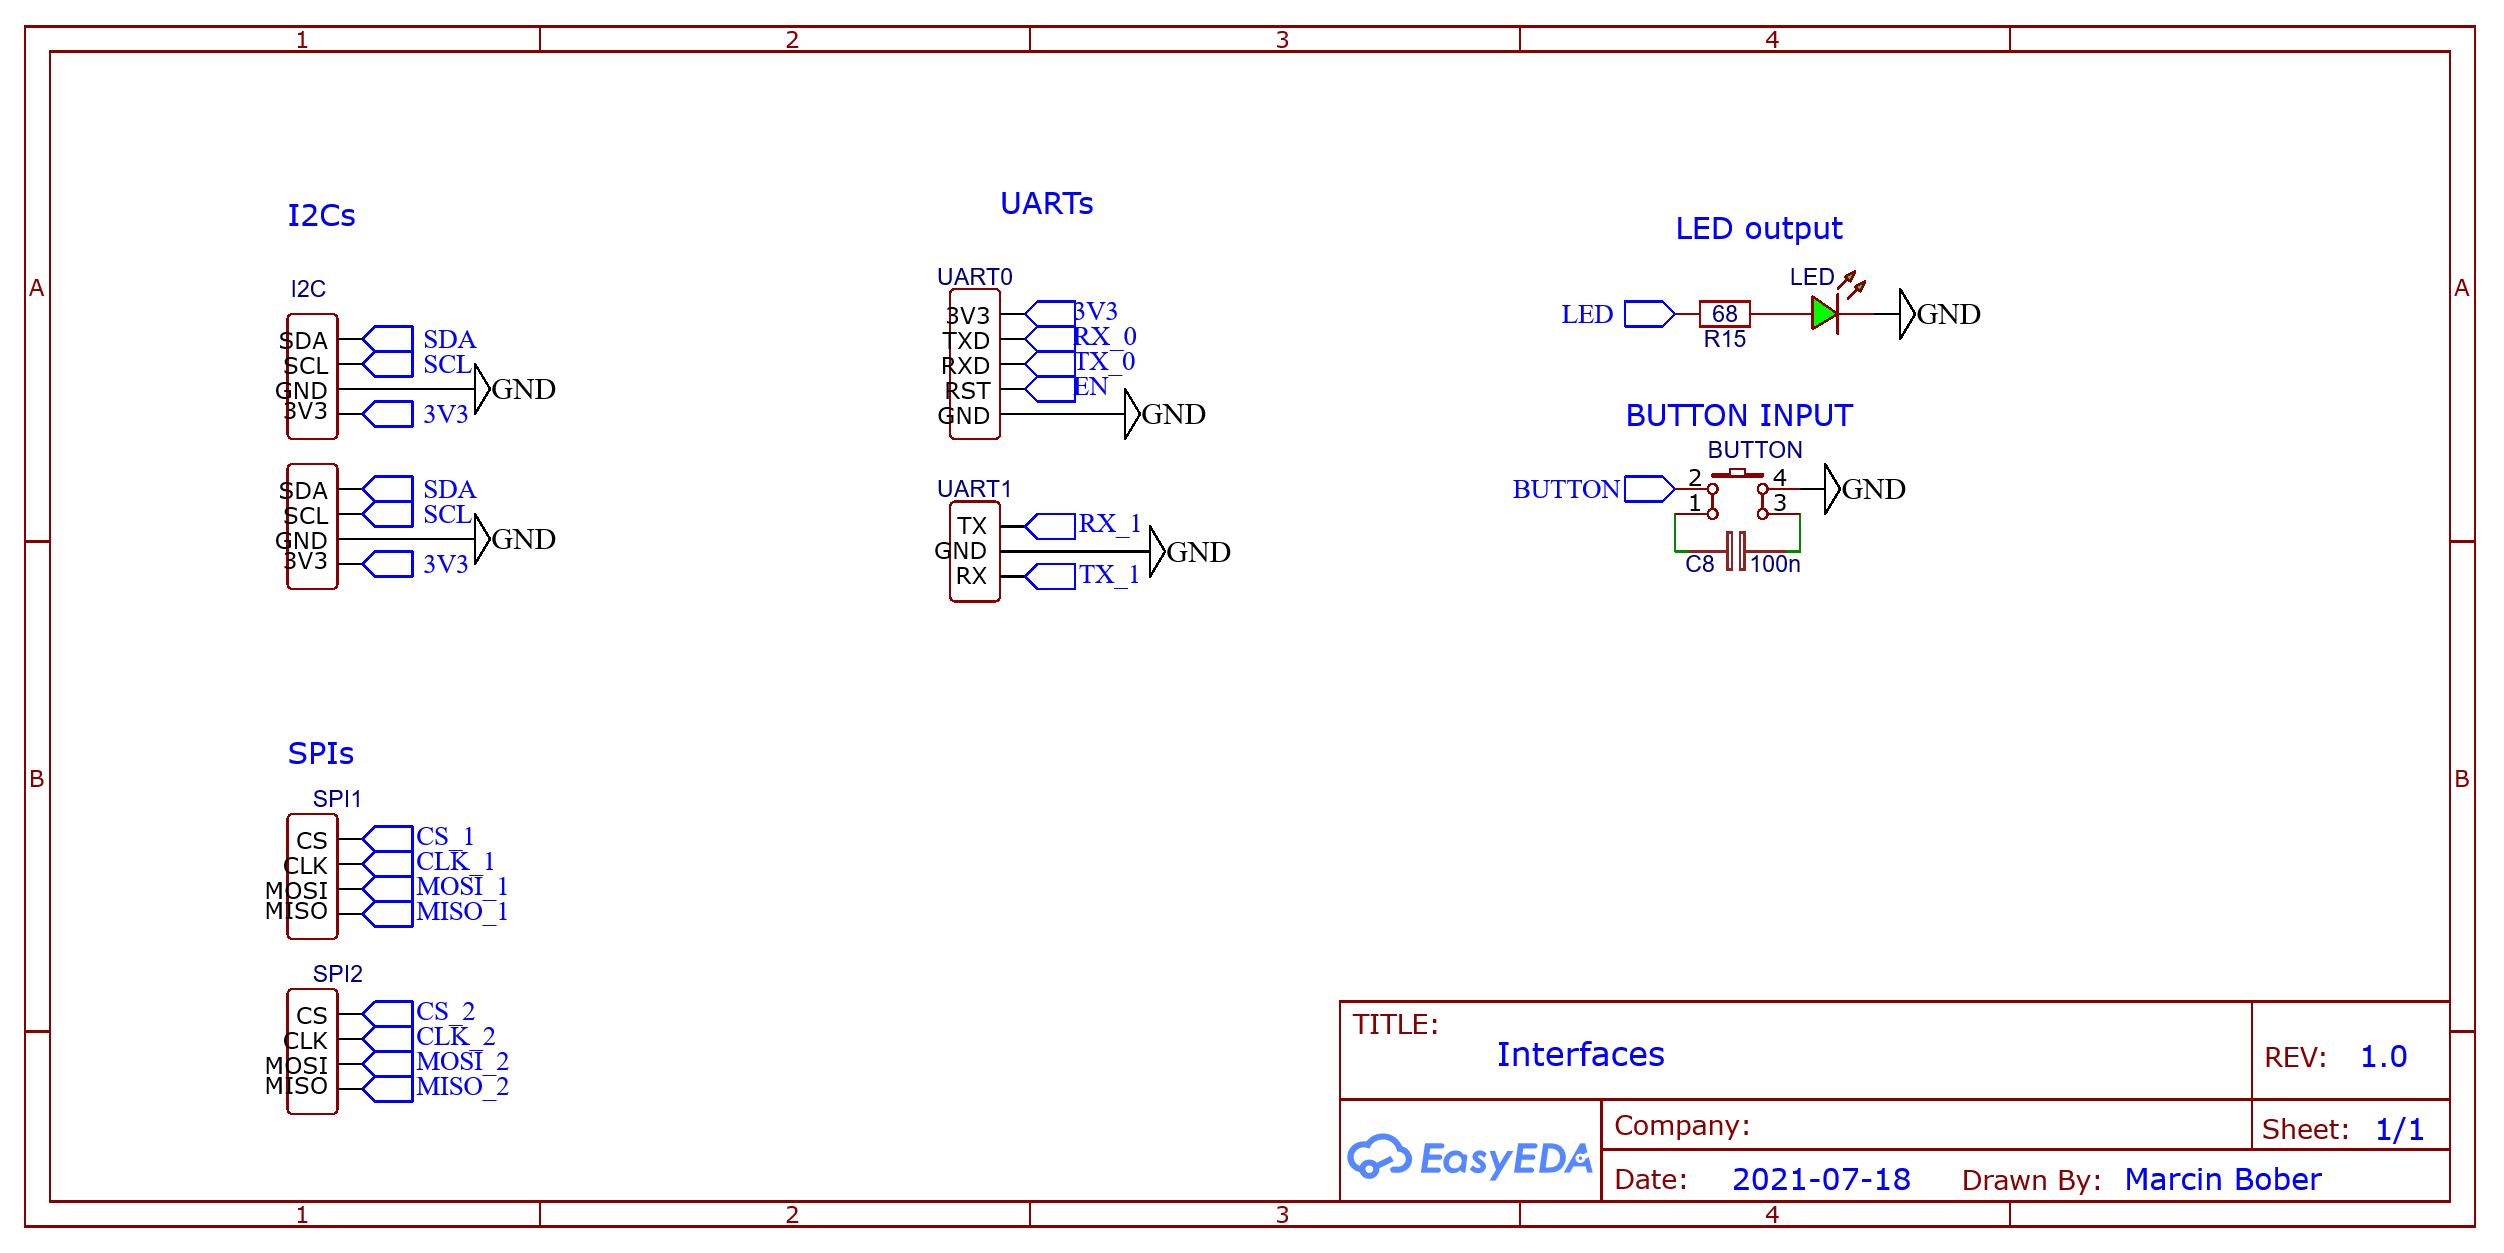
\includegraphics[width=0.85\textwidth]{img/pcb3.png}
                      \caption{Schemat płytki PCB (interfejsy)}
                      \label{fig:pcb_schematic_3}
                    \end{figure}
                \end{landscape}